\section{\label{sec:level1}Atomic Magnetometers}
Atomic, or as they are also often referred to as optical, magnetometers are devices which determine the local magnetic field by measuring the Larmor precession by optically probing a specific atomic transition \citep{Kitching2008MicrofabricatedApplications}. Larmor precession occurs due to the magnetic moment of particles, such as electrons and atomic nuclei, experiencing a torque when a magnetic field is applied. The Larmor frequency is given by: 

\begin{equation}
\label{eq:interactionham0}
\omega_{L}=\gamma B,
\end{equation}
%The interaction Hamiltonian is $H_{int}=\vec{\mu}\cdot\vec{B}$ for either particle.
where the gyromagnetic constant, $\gamma$, is the ratio of the magnetic moment, $\vec{\mu}$ to the total angular moment, $\vec{J}$. The magnitude of the magnetic field is given by $B$ \citep{Kitching2011AtomicReview}. Since electrons are fermions, the magnetic moment occurs due to the $\frac{1}{2}$- spin properties of the particles. In addition the atomic nucleus has a smaller magnetic moment, $\vec{\mu}_I$, resulting from the nuclear spin, $\vec{I}$ \citep{Foot2005AtomicPhysics}. Since the valence electron and nucleus form a coupled system for alkali atoms, $B$ results in precession of the electron spin which also forces the nuclear spin to rotate in the same direction \citep{Seltzer2008AtomicMagnetometery}. 

\subsection{Alkali Atomic Structure}
\begin{figure}[b]
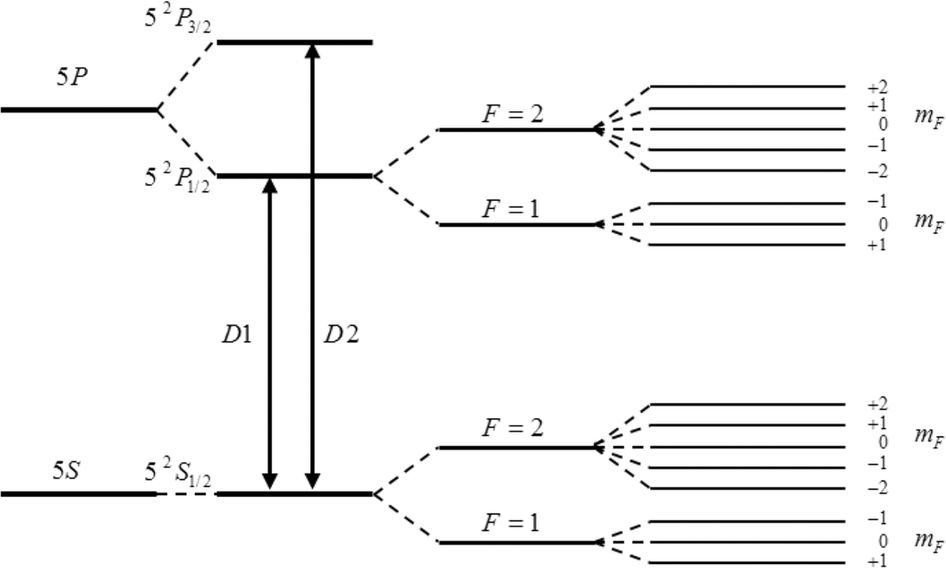
\includegraphics[height=0.25\textwidth,keepaspectratio,]{zeemspec}
\caption{\label{fig:zeemspec}Spectroscopic structure of alkali metal ($^{87}Rb$) atoms with $m_{F}$ degeneracy lifted. The hyperfine and Zeeman sublevels of the second excited state are omitted \citep{Li2017EllipticalVapor}.}
\end{figure}

It is useful to initially consider the atomic energy structure alkali atoms as shown in Fig. (\ref{fig:zeemspec}). The fine structure arises from relativistic effects of the electron spin-orbit interaction. For the same principle quantum number $n$, there is a shift in energy for different values of $J$ \citep{Steane2002AtomicMatter}. The total angular momentum of the valence electron is: 

\begin{equation}
\label{eq:interactionham0}
\vec{J}=\vec{L}+\vec{S}, 
\end{equation}


where $\vec{S}$ is the electron spin angular momentum and $\vec{L}$ is the orbital angular momentum. When the valence electron is in the ground state, $\vec{L} = 0$. When the electron is in the first excited state, $\vec{L}=1$. The spectroscopic notation used is $n^{2S+1}L_{J}$ for the fine structure where the $\vec{L} = 0, 1, ...$ is associated with the $'S','P',...$ shell letters. The energy transitions between the ground 'S' state and the excited 'P' states are known as $D$-line transitions as shown in Fig. (\ref{fig:zeemspec}) \citep{Foot2005AtomicPhysics,LandiDeglInnocenti2014AtomicProcesses}.  

The hyperfine energy splitting occurs due to the interaction between the spin of the atomic nucleus and the electron spin. The total atomic angular momentum is:

\begin{equation}
\label{eq:interactionham0}
\vec{F}=\vec{I}+\vec{J},
\end{equation}
\\
where $\vec{F}$ points parallel to $\vec{J}$. $\vec{I}$ is the sum of the proton and neutron $\frac{1}{2}$-spin particles for a specific isotope \citep{LandiDeglInnocenti2014AtomicProcesses}. The Zeeman effect occurs in the presence of a magnetic field and results in further energy splitting of $\Delta E_{L}=\hbar\omega_{L}$ into Zeeman sublevels $m_{F}=\{-F,-F+1 ... F-1,F\}$ \citep{Seltzer2008AtomicMagnetometery}. 

\subsection{Pumping and Probing} 

\begin{figure}[b]
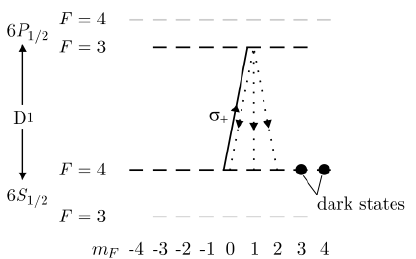
\includegraphics[height=0.3\textwidth,keepaspectratio,]{opticalpumping}
\caption{\label{fig:pumprobe} $\sigma_{+}$ beam pumping atoms into the Dark states \citep{Birzhandi2013EffectPhenomenon}.}
\end{figure}
 \begin{figure}[t]
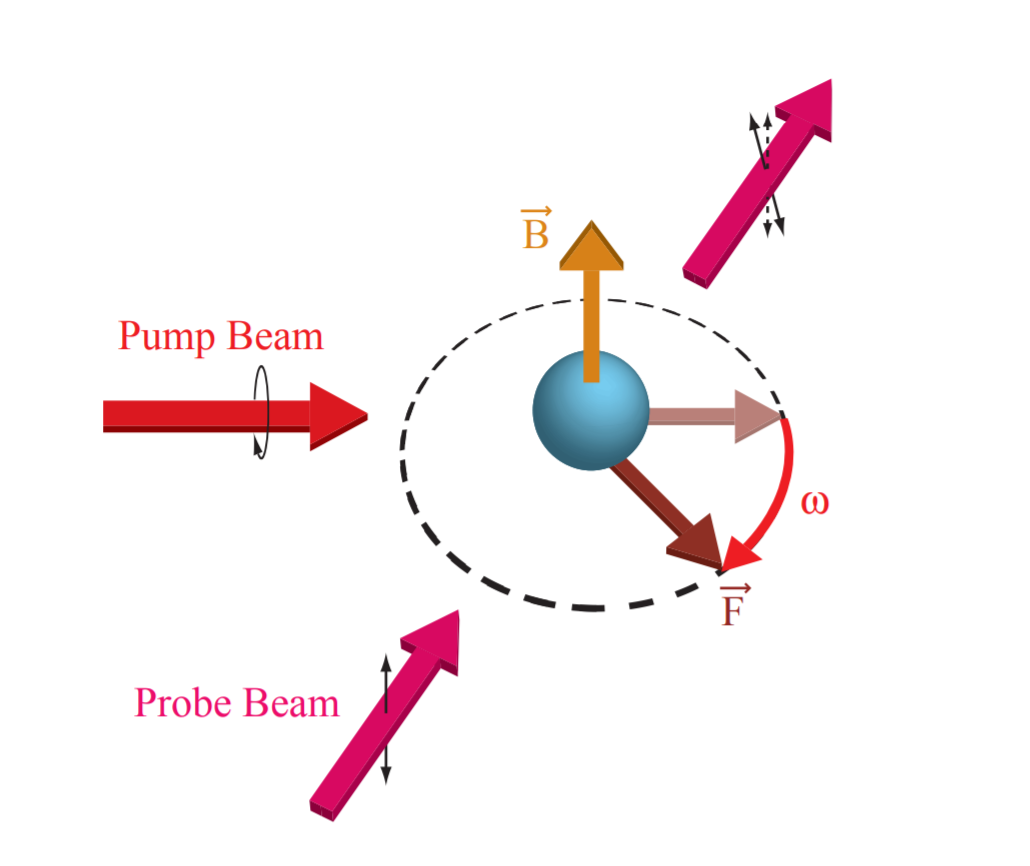
\includegraphics[height=0.3\textwidth,keepaspectratio,]{pumprobe}
\caption{\label{fig:opticalpumping} Schematic diagram of a pump-probe atomic magnetometer scheme. The circularly polarised pump beam produces a polarisation orientation of the atomic spins in the direction of laser propagation. In the presence of a weak magnetic field the angular momentum of the atom precesses at $\omega_{L}$ around $\vec{B}$. The output linearly polarised probe has undergone a plane rotation angle corresponding to the component of $\vec{S}$ in that direction \citep{Seltzer2008AtomicMagnetometery}.}
\end{figure}

The evolution of the valence electron spin of the alkali atoms can be used to detect weak $B$ fields. A circularly polarised beam is used align the valence electron spin, such that the atomic vapor becomes magnetised \citep{Sander2012MagnetoencephalographyMagnetometer.}. Circularly polarised light which is resonant with the D1 transition line pumps atoms into Dark states and produces a polarisation of the atomic spin parallel to the direction of propagation of the applied field \citep{Groeger2006AMagnetometer}. $\sigma^{+}$ polarised light excites atoms from a hyperfine ground state to the hyperfine exited $P_{\frac{1}{2}}$ state where $m_{F}$ is increased by +1  \citep{Birzhandi2013EffectPhenomenon}. The atomic selection rules \citep{Steane2002AtomicMatter} dictate that the atom can spontaneously decay to the $\ket{S_{\frac{1}{2}}, m_{F}=\{-1,0,1\}}$ states. If this transition is continually pumped the atoms will be transferred into Dark states which are optically transparent to the incoming laser photons. As shown in Fig. (\ref{fig:opticalpumping}) since there is no possible excited state transition.      

When all the atoms are transferred to Dark states the maximum transmission of photons through the cell is detected. The Larmor precession of the atomic spin around $\vec{B}$ results in a phase accumulation. Various detection methods have been implemented including detecting the modulation of the pump light transmission intensity and phase when a static $B_{0}$ field is applied at 45$^{\circ}$ to the pump beam and a radio frequency (rf) magnetic field $B_{1}(t)$ resonant with $\omega_{L}$ is applied perpendicular to $B_{0}$ \citep{Schwindt2007Chip-scaleTechnique,Groeger2006AMagnetometer}. Additionally, the output rotation angle of a linearly polarised probe laser is related to the degree of $\vec{S}$ in that direction  \citep{XiaMagnetoencephalographyMagnetometer,Kominis2003AMagnetometer}. The advantage of this scheme compared to the rf AM scheme is that the laser intensity noise is reduced and small angle polarisation rotations can be detected \citep{Budker2007OpticalMagnetometry}.  

The combination of homogeneous, natural and pressure, broadening of the transition linewidth and Doppler broadening of alkali metal atoms contained in a vapor cell results in a Voigt lineshape. At room temperature, the Doppler broadening linewidth is $\approx 0.5$ GHz for a alkali metal vapor cell \citep{Yariv2006PhotonicsCommunications,Siddons2008AbsoluteExperiment}. The ability to resolve transitions between hyperfine levels depends on the degree of Doppler broadening in comparison to the hyperfine $F \rightarrow F^{'}$ transition frequency. Transitions between a $F$ ground state and $F^{'}$ excited state can be driven using a dichroic atomic vapor laser lock (DAVLL) where the frequency stabilisation is $\approx 1$ MHz/h \citep{Bison2004DevelopmentCardio-magnetometer,Imanishi2005FrequencyCell}. 

\subsection{Sensitivity}
Initially the AM signal-to-noise ratio (S/N) was the limited by the $B$ field detection sensitivity. To increase the signal, the density of atoms in the vapor was increased \citep{Kitching2011AtomicReview}. However, as the atomic density was increased the number of collision events increased. The coherence time $T_{2}$ of the atomic spin is limited by atom collisions with the cell walls and atom-atom collisions. Complete depolarisation of the atomic spin occurs when alkali atoms collide with the cell walls or buffer gas atoms \citep{Budker2007OpticalMagnetometry}. The spin-exchange interaction occurs when alkali metal atoms have collisions with other alkali atoms. The spin-exchange interaction occurs rapidly such that the nuclear spin is unaffected. The total spin of the particles $\vec{S}=\vec{S}_{1}+\vec{S}_{2}$ is conserved but at least one spin value will change \citep{Happer1977EffectVapors}. The decoherence of the alkali spin influences the fundamental measurement sensitivity of an atomic magnetometer as: 

\begin{equation}
\label{eq:interactionham0}
\delta B =\frac{1}{\gamma\sqrt{N T_{2} t}},
\end{equation}

which is shot-noise limited \citep{Kominis2003AMagnetometer}. The measurement duration time and the number of alkali metal atoms are given as $t$ and $N$, respectively. 

\subsection{SERF magnetometer}
The development of the alkali-alkali spin-exchange relaxation-free (SERF) technique is demonstrated experimentally in Ref.[\citen{Allred2002High-SensitivityRelaxation}] to increase the magnetometer's sensitivity. The concept initially appears counterproductive to reducing transition broadening. Firstly the potassium atomic number density in the vapor cell to increased to $n = 10^{14}$ cm$^{3}$ thereby increasing the spin-relaxation rate to $T_{2}$ > 1/$\omega_{L}$. In this regime the two hyperfine ground states are described as being "locked" together and precesses slowly around a small, near zero, $B_{y}$ field in the direction of the highest occupation $F$ state. Transition broadening now is limited by collisions where $\vec{S}$ is not conserved, but the rate of these collisions is small comparatively. The theoretically achievable shot-noise limited sensitivity is $2 \times 10^{-18}$ THz$^{-1/2}$ and the measured sensitivity is 10 fTHz$^{-1/2}$ which is limited by current fluctuation noise from the magnetic shielding. The SERF technique can eliminate alkali-alkali spin-relaxation when measuring magnetic fields up to $\approx10$ nT \citep{Budker2007OpticalMagnetometry}. In Ref. [\citen{Kominis2003AMagnetometer}] using the SERF technique, the 0.54 fTHz$^{-1/2}$ sensitivity of the atomic magnetometer is demonstrated for a vapor cell of volume 0.3 cm$^{3}$ where measurement of the probe beam polarisation was achieved using a multi-channel photodiode. 